\documentclass{article}
\input{/DocHeader.tex}
\title{CPSC 540 --- Assignment 1}
\author{Aaron Berk}
\begin{document}
\maketitle


\section{Fundamentals}
\label{sec:fundamentals}


\subsection{Matrix notation}
\label{sec:matrix-notation}

\begin{enumerate}
\item $f(w) = w^Ta + \alpha + \sum_{j=1}^d w_ja_j.$
  \begin{align*}
    \nabla_w f(w) &= \nabla ( 2\ip{w, a} + \alpha) = 2a
    \\
    \nabla_w^2 f(w) &\equiv 0
  \end{align*}
\item $f(w) = a^Tw + a^TAw + w^TA^Tb.$
  \begin{align*}
    \nabla_w f(w) %
    %= \nabla \big( \ip{a, w} + \ip{a, Aw} + \ip{Aw, b}\big) %
    &= \nabla_w \big( \ip{a, w} + \ip{w, A^Ta} + \ip{w, A^T b}\big) %
    % = a + A^Ta + A^T b %
    = a + A^T(a + b)
    \\
    \nabla_w^2 f(w) %
    &\equiv 0
  \end{align*}
\item $f(w) = w^Tw + w^TX^TXw + \sum_{i=1}^d\sum_{j=1}^d w_iw_ja_{ij}.$
  \begin{align*}
    f(w) &= \|w\|_2^2 + \|Xw\|_2^2 + w^T A w
    \\
    \implies \quad %
    \nabla_w f(w) &= 2(1+ X^TX)w + (A + A^T)w
    \\
    \nabla_w^2 f(w) &= 2(1+ X^TX) + A + A^T
  \end{align*}
\item $f(w) = \frac{1}{2}\sum_{i=1}^n v_i(w^Tx^i - y^i)^2 + \frac{\lambda}{2}\|w\|^2.$
  \begin{align*}
    f(w) &= \frac{1}{2} (Xw - y)^T V (Xw - y) + \frac{\lambda}{2} \|w\|^2
    \\
    \implies \quad \nabla_w f(w) %
         &= 2 X^T V (Xw-y) + \lambda w
    \\
    \nabla_w^2 f(w) %
         &= 2 X^T V X + \lambda I
  \end{align*}
\item $f(w) = - \sum_{i=1}^n \log p(y^i | x^i w) + \frac{1}{2}\sum_{j=1}^d
  b_jw_j^2;\quad p(y^i \mid x^i, w) = \Phi(y^i w^T x^i).$
  \begin{align*}
    \nabla_w f(w) %
    &= - \sum_{i=1}^n \frac{\phi(y^i w^T x^i)}{\Phi(y^i w^T x^i)}y^i x^i
      + Bw
    \\
    \nabla_w^2 f(w) %
    &= - \sum_{i=1}^n y^ix^i \partial_w \frac{\phi(y^i w^T x^i)}{\Phi(y^i w^T
      x^i)}
    = \sum_{i=1}^n x^i(x^i)^T \frac{\phi^2 (y^i w^T x^i ) - y^i w^T x^i \phi(y^i w^T x^i)
      \Phi(y^i w^T x^i )}{\Phi^2 (y^i w^T x^i)}
  \end{align*}

\end{enumerate}


\subsection{Regularization and cross-validation}
\label{sec:regul-cross-valid}

\begin{enumerate}
\item

  \lstinputlisting{./a1/leastSquaresRBFL2.m}

  \begin{figure}[h]
    \centering
    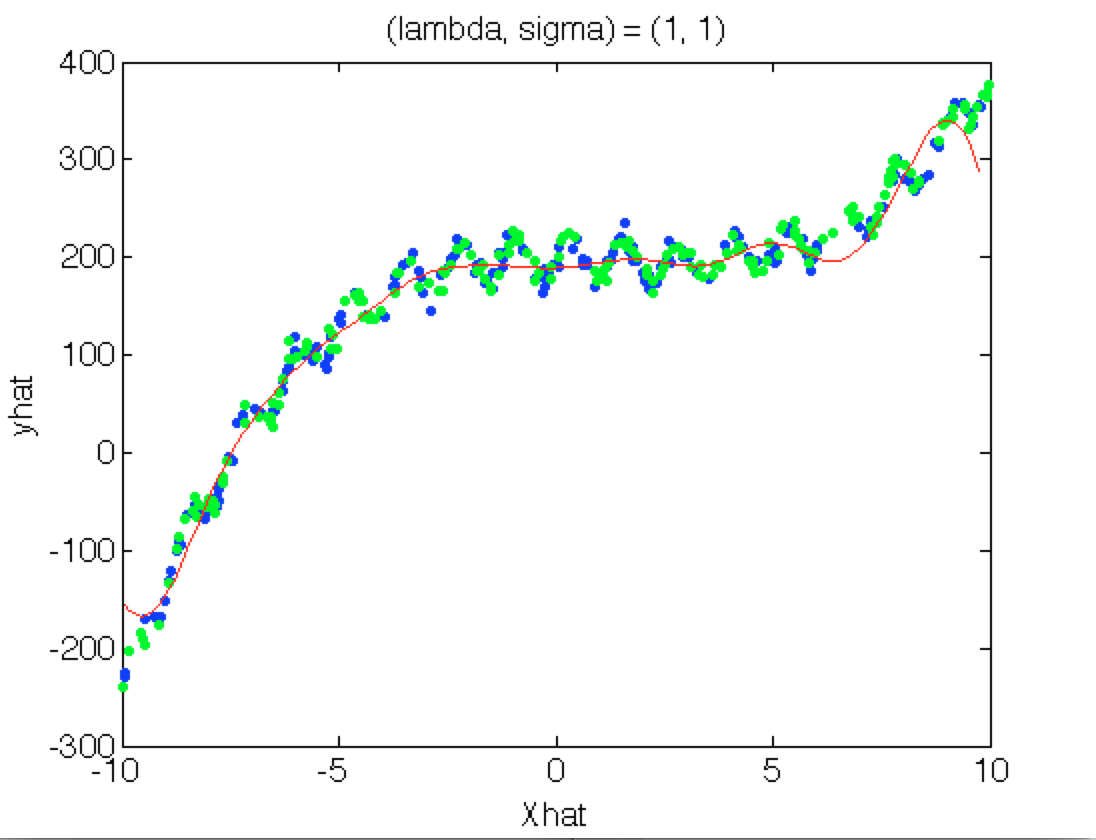
\includegraphics[width=.5\textwidth]{./fig/nonlinearLS-121.png}
    \caption{Plot of {\color{blue}training data}, {\color{green}test data} and {\color{red}approximation
      to test data} derived as the solution to the $L^2$-regularized NLS
      problem. Output: \texttt{squaredTestError = 636.0074}.}
    \label{fig:rbfnonlinear}
  \end{figure}
\item What is the cost in big-O notation of
training the model on $n$ training examples with $d$ features under (a) the linear basis, and (b) Gaussian
RBFs (for a fixed $\sigma$)? What is the cost of classifying $t$ new examples under these two bases? Assume
that multiplication by an $n\times d$ matrix costs $O(nd)$ and that inverting a
$d\times d$ linear system costs $O(d^3)$.
\item Hand in your cross-validation procedure and the plot you obtain with the
  best values of $\lambda$ and $\sigma$.

  Using the grid
\begin{verbatim}
lambda = logspace(-7, -5, 30);
sigma = logspace(-1,0,30);
\end{verbatim}
  the best $\lambda$ and $\sigma$ found were
  $(\lambda, \sigma) = (4.894\times 10^{-7}, 0.7279)$ giving a mean-squared test
  error on the test set of $59.956$.
  
  \lstinputlisting{./a1/gridSearchCV.m}

  \begin{figure}[h]
    \centering
    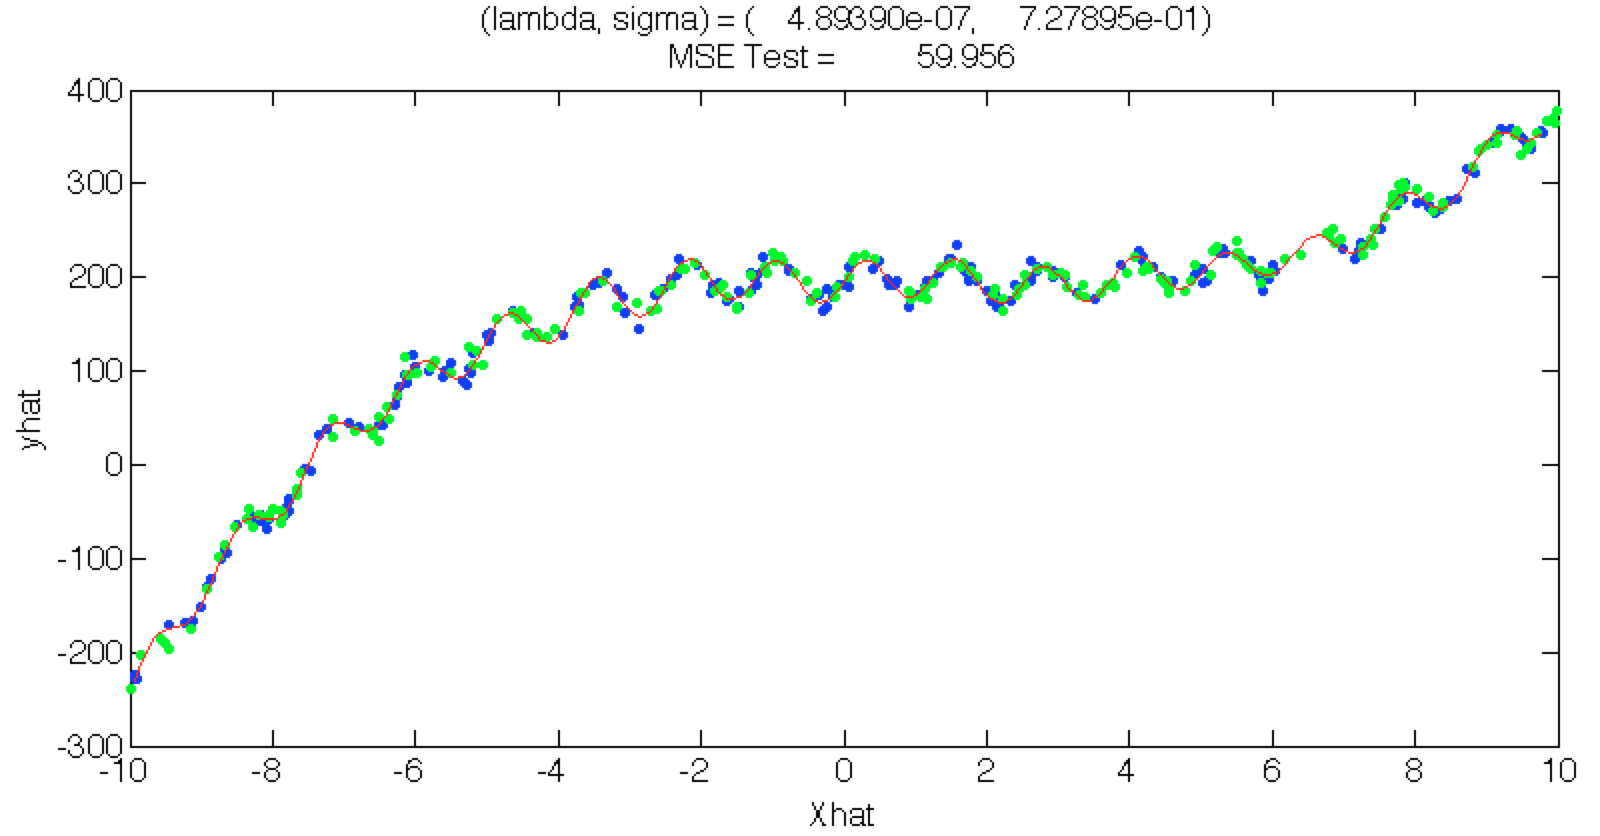
\includegraphics[width=.65\textwidth]{./fig/nonlinearLS-123.png}
    \caption{the best $\lambda$ and $\sigma$ found were
      $(\lambda, \sigma) = (4.894\mathrm\times 10^{-7}, 0.7279)$ giving a mean-squared test
      error on the test set of $59.956$. Colours correspond to train, test,
      predict as above.}
    \label{fig:rbfnonlinearcv}
  \end{figure}
\end{enumerate}

\subsection{MAP estimation}
\label{sec:map-estimation}

For each of the alternate assumptions below, write it in the “loss
plus regularizer” framework
\begin{enumerate}
\item Laplace distribution likelihoods and priors,
  \begin{align*}
    y^i \sim \mathcal{L}(w^T x^i, 1), \quad w_j \sim \mathcal{L}(0, \lambda^{-1})
  \end{align*}
  \soln

  This implies that
  \begin{align*}
    p( y^i \mid x^i, w) = \frac{1}{2} \exp(-|w^T x^i - y^i| ), \qquad p(w_j) =
    \frac{\lambda}{2} \exp ( -\lambda |w_j|)
  \end{align*}
  Computing the negative log-likelihood function then gives
  \begin{align*}
    L(y^i \mid x^i) = - \log \frac{1}{2} - \log \frac{\lambda}{2} + |w^T x^i -
    y^i| + \frac{\lambda}{2} \|w\|_1 
  \end{align*}
  Hence, the function for the associated convex problem is given by 
  \begin{align*}
    f(w) = \|Xw - y\|_1 + \lambda \|w\|_1
  \end{align*}

  
\item Gaussians with separate variance for each training example and variable,
  \begin{align*}
    y^i \sim \mathcal{N}(w^Tx^i, \sigma_i^2), \quad w_j \sim \mathcal{N}(0, \lambda_j^{-1}).
  \end{align*}
  \soln

  Using the same process as above, the function for the associated convex
  problem is given by
  \begin{align*}
    f(w) = (Xw - y)^T \Sigma^{-1} (Xw - y) + w^T \Lambda w, \quad \Sigma &=
    \mathrm{diag}\,(\sigma_i^2), \\\Lambda &= \mathrm{diag}\,(\lambda_j)
  \end{align*}
\item Poisson-distributed likelihood (for the case where $y^i$ represents discrete counts) and Gaussian prior,
  \begin{align*}
    y^i \sim \mathcal{P}(\exp(w^T x^i)), \quad w_j \sim \mathcal{N}(0, \lambda^{-1})
  \end{align*}
  \soln

  Unpacking the definition of the distribution of $y^i$, it follows that the
  conditional probability for $y^i$ and it's negative conditional
  log-likelihood are given by 
  \begin{align*}
    p(y^i \mid x^i, w) &= \frac{\exp(y^i w^T x^i)\exp(-\exp(w^T x^i))}{(y^i)!}\\
    -\log p(y^i \mid x^i, w) &= \log((y^i)!) - y^i w^T x^i + \exp(-w^T x^i)
  \end{align*}
  Hence, the associated convex function is given by
  \begin{align*}
    f(w) = \log (y!) + YXw + \exp(-Xw) + \frac{\lambda}{2} \|w\|_2^2, \qquad z!
    &:= z_1!\,z_2!\,\cdots z_n!,\\ Y &:= \mathrm{diag}\,(y^i)
  \end{align*}




\end{enumerate}

\section{Convex functions}
\label{sec:convex-functions}

\subsection{Minimizing strictly-convex quadratic functions}
\label{sec:minim-strictly-conv}

\begin{enumerate}
\item We seek the orthogonal projection of $v$ onto $\reals^n$: $\argmin_{w\in
    \reals^n} f(w) := \|w - v\|_2^2$. Notice that this is equal to $(\Re
  v_j)_{j=1}^n =: \Re v$. 
\item Assume $f(w) := \frac{1}{2} \|Xw - y\|_2^2 + \frac{1}{2} w^T \Lambda
  w$. We want to find $w^* := \argmin_w f(w)$. Taking derivatives, as the
  objective is smooth:
  \begin{align*}
    \partial_j f(w) = \partial_j \big( \frac{1}{2}\ip{Xw, Xw} - \ip{Xw, y} \big) +
    \lambda_j w_j = (X^T X w)_j - (X^T y)_j + \lambda_j w_j  = 0
  \end{align*}
  implying that
  \begin{align*}
    w = (\Lambda + X^T X)^{-1} (X^T y)
  \end{align*}
  
\item $\partial_j f(w) = \sum_{i=1}^n v_i (w_j x_{ij} - y_i)x_{ij} +
  \lambda (w_j - w^0)$

  $0 = v^T X w - X^T \mathrm{diag}(v_i) y + \lambda (w-w^0)$ implying that $w =
  (v^TX + \lambda)^{-1} (\lambda w^0 + X^T \mathrm{diag}(v_i) y)$
\end{enumerate}

\clearpage
\section{Numerical Optimization}
\label{sec:numer-optim}

\subsection{Gradient descent and Newton's method}
\label{sec:grad-desc-newt}

Report the effect on performance (in terms of number of backtracking iterations
and total number of iterations) of making the following changes to
\texttt{findMin}:
\begin{enumerate}
\item When backtracking, replacing the cubic-Hermite interpolation with the
  simpler strategy of dividing $\alpha$ in half (as suggested in the Boyd \&
  Vandenberghe book).
\item Instead of resetting $\alpha$ to one after the line-search, set it using
  the Barzilai-Borwein step-size, given by
    \[
      \alpha \leftarrow -\alpha\frac{v^T\nabla f(w)}{v^Tv},
    \]
    where $v$ is the new gradient value minus the old gradient value.\\
  \item Fix the step-size $\alpha$ to $1/L$, where $L$ is given by
    \[
      L = \frac{1}{4}\max\{\text{eig}(X^TX)\} + \lambda,
    \]
    which is the Lipschitz constant of the gradient.
  \item Instead of using the gradient direction, set $d$ to the Newton
    direction which is given by
    \[
      d = [\nabla^2 f(w)]^{-1}\nabla f(w).
    \]
  \end{enumerate}
  For the Newton direction, you'll need to make a new objective function that
  returns the Hessian in addition to the function and gradient, and modify
  \emph{findMin} to use the Hessian.


  \textbf{The Student's answer:}

\begin{tabular}[h]{cccc}
  \textbf{Method} & \textbf{funEvals} & \textbf{backtracks} & \textbf{time (sec)}\\
  Cubic Hermite & 23 & 13 & 0.049378\\
  $\alpha \mapsto \alpha/2$ & 83 & 69 & 0.130050\\
  Barzilai-Borwein & 21 & 8 & 0.034763\\
  Lipschitz & 35 & 0 & 0.058531\\
  Newton & 5 & 0 & 0.009681
\end{tabular}

\clearpage
\subsection{Hessian-free Newton}
\label{sec:hessian-free-newton}

Use Matlab's \texttt{pcg} function to implement a ``Hessian-free" Newton's
method, where you use conjugate gradient to solve the Newton system. Report the
output of \texttt{findMin} on \texttt{rcv1\_train\_binary.mat} when using this
strategy and using \texttt{optTol} as the tolerance for \texttt{pcg}.

\textbf{The Student's answer:}
\begin{verbatim}
pcg converged at iteration 12 to a solution with relative residual 0.0071.
pcg converged at iteration 9 to a solution with relative residual 0.0089.
     2      0     1.00000e+00     5.18715e+03     6.38540e+01
pcg converged at iteration 9 to a solution with relative residual 0.0071.
     3      0     1.00000e+00     4.22805e+03     1.80539e+01
pcg converged at iteration 8 to a solution with relative residual 0.0088.
     4      0     1.00000e+00     4.09305e+03     1.02721e+01
pcg converged at iteration 8 to a solution with relative residual 0.0053.
     5      0     1.00000e+00     4.08556e+03     2.29591e+00
pcg converged at iteration 8 to a solution with relative residual 0.008.
     6      0     1.00000e+00     4.08547e+03     4.88609e-02
pcg converged at iteration 9 to a solution with relative residual 0.0091.
     7      0     1.00000e+00     4.08547e+03     7.96543e-05
Problem solved up to optimality tolerance
Elapsed time is 1.493054 seconds.
\end{verbatim}

\subsection{Multi-class logistic regression}
\label{sec:multi-class-logistic}

Hand in the code and report the validation error



\end{document}

%%% Local Variables:
%%% mode: latex
%%% TeX-master: t
%%% End:
